% Also note that the "draftcls" or "draftclsnofoot", not "draft", option
% should be used if it is desired that the figures are to be displayed in
% draft mode.
\documentclass[3p,authoryear]{elsarticle}
%
%
%
%		Packages
%
%
\usepackage{subfigure}
\usepackage{amsmath}
\usepackage{amsthm}
\usepackage{amsfonts} 
\usepackage{amssymb}
\usepackage{verbatim}
\usepackage{enumerate}
\usepackage[acronym=true]{glossaries} 
\usepackage{algorithm}
\usepackage[noend]{algpseudocode}
\usepackage{xcolor}
\usepackage[colorlinks=true]{hyperref}
\usepackage{url}
\usepackage{subfigure}
\usepackage{xspace}
\usepackage{booktabs}
\usepackage{microtype}


%
% 
% 
%
\newcommand{\Ord}{\mathcal{O}}
\newcommand{\Orlib}{{\sc or-library}\xspace}
\newdefinition{definition}{Definition}

\newcommand{\CBGAe}{\gls{CBGA}$^d_\epsilon$\xspace}

\algnewcommand{\IfThen}[2]{% \IfThenElse{<if>}{<then>}{<else>}
  \State \algorithmicif\ #1\ \algorithmicthen\ #2}
%
%
%
%		Glossary entries
%
%
%
\newacronym{GA}{GA}			{\textit{Genetic Algorithm}}
\newacronym{MKP}{MKP}	    {\textit{Multidimensional Knapsack Problem}}
\newacronym{CBGA}{CBGA}		{\textit{Chu \& Beasley Genetic Algorithm}}

%
%
%
%		Beginning
%
% 

\begin{document}

\begin{frontmatter}
\title{A randomized heuristic repair based on efficiency groups for the 0-1 multidimensional knapsack problem}

\title{Efficiency groups and a randomized heuristic repair for the 0-1 multidimensional knapsack problem}

\author{Jean P. Martins\corref{cor1}}
\ead{jeanmartins@utfpr.edu.br}
\cortext[cor1]{Corresponding author}

%\author[ufabc]{Claudio Meneses}
%\ead{}


\address{Federal University of Technology Paran\'a, Academic Department of Informatics, Pato Branco--PR, Brazil}
%
%
%
%		Abstract
%
%
\begin{abstract}
The multidimensional knapsack problem (MKP) is an NP-hard combinatorial optimization problem whose solution consists of determining a subset of items of maximum total profit that does not violate capacity constraints. Due to its hardness, large-scale MKP instances are usually a target for metaheuristics, a context in which effective feasibility maintenance strategies are crucial. In 1998, Chu and Beasley proposed one of the most successful repair heuristics which is still employed in more recent metaheuristics. However, due to its deterministic nature, the diversity of solutions such heuristic provides is not sufficient for long runs. As a result, the search ceases to find new solutions after a while. This paper proposes an efficiency-based randomization strategy for the heuristic repair which increases the variability of the repaired solutions, without deteriorating quality and improves the overall results. We compared our randomized heuristic repair against the original one in 270 \Orlib instances, with better results found in runtime and solution quality. 
\end{abstract}
%
%
%
%		Keywords
%
%
\begin{keyword}
knapsack problem, heuristic repair, evolutionary algorithms, metaheuristics
\end{keyword}

\end{frontmatter} 
\glsresetall 
\newcommand{\x}{\boldsymbol{x}}

\section{Introduction} 


%
%					The Multidimensional Knapsack Problem
%

\glsreset{MKP}
The \gls{MKP} is a well-known strongly NP-Hard combinatorial optimization problem~\citep{freville2004, puchinger2010mkp}. To solve an instance of the \gls{MKP} one must choose choose, from a set of $n$ items, a subset that yields the maximum total profit. Every item chosen contributes with a profit $p_j > 0$ ($j=1,\dots,n$) but also consumes $w_{ij}$ from the amount of resources available $r_i>0$ ($i=1,\dots, m$). Therefore, a solution is \textit{feasible} only if the total of resources it consumes do not surpass the amount available. By representing solutions as $n$-dimensional binary vectors, the \gls{MKP} is formulated as:
\begin{alignat*}{3}
\max   \quad& f(\x) = \sum_{j=1}^{n} p_j x_j, &  \\
\text{subject to} \quad& \sum_{j=1}^{n} w_{ij} x_j \leq r_i &\quad i=1,\dots,m,\\
                      & x_j\in\{0,1\}, &\quad j=1,\dots,n.
\end{alignat*}


The \gls{MKP} is considerably harder than its unidimensional counterpart, not admitting an efficient polynomial-time approximation scheme even for $m=2$~\citep{Kulik2010}. Furthermore, \gls{MKP} hardness increases with $m$, and larger instances still cannot be effectively solved to optimality~\citep{mansini2012}. Due to these limitations, metaheuristics have been the most successful alternatives to solve the largest instances available at the \Orlib\footnote{\url{http://people.brunel.ac.uk/~mastjjb/jeb/info.html}}. However, most of the best known solutions for such instances were attained by hybrid methods encompassing tabu search, evolutionary algorithms, linear programming and branch and bound~\citep{puchinger2010mkp}.

%One of the earliest references concerning \glspl{MKP} was a dynamic programming approach proposed by Gilmore and Gomory~\cite{gilmor1966}, which was further extended by Weingartner and Ness~\cite{weingartner1967} by embedding heuristics to the algorithm. Branch-and-bound was also used to improve dynamic programming approaches, as proposed by Marsten~\cite{marsten1977,marsten1978}. In the same context, Shih~\cite{shih1979branch} proposed the first branch-and-bound implementation based on linear programming. However, due to high space requirements and the limited computational capacity, such approaches were limited to very small problems. In order to circumvent such limitations, Gavish and Pirkul~\cite{gavish1985} developed a branch-and-bound using rules to reduce the problem size, obtaining better results than Shih's method. A more recent approach based on an approximated dynamic programming was proposed by Bertsimas~\cite{bertsimas2002}, while a hybridization with a branch-and-cut-procedure was proposed by Boyer~\cite{boyer2009}.

% Tabu-search methods, as developed by Glover and Kochenberger~\cite{glover1996} and further improved by Hanafi and Freville~\cite{hanafi1998} in 1998, were able to solve to optimality all the public instances available so far~\cite{freville2004}. 
 
\cite{chu1998} results can be considered a landmark regarding metaheuristics for the \gls{MKP}. The method they proposed, which we refer to as \gls{CBGA}, was the first metaheuristic to deal with large-scale \gls{MKP} instances and influenced many posterior analysis, see for example~\cite{gottlieb2000b,gottlieb2001} and \cite{tavares2006,tavares2008}. Additionally, the heuristic repair employed by \gls{CBGA} has proved itself as one of the most effective alternatives for feasibility maintenance and it is commonly employed by other metaheuristics, see~\cite{kong2008},\cite{wang2012,wang2012b}, \cite{martins2013a,martins2013}, \cite{chih2014} and \cite{azad2014}. %And last, the set of instances used to assess \gls{CBGA}'s performance became a standard benchmark for metaheuristics. 

\textcolor{red}{
Several of \gls{CBGA} results have been improved or matched by many algorithms. Amongst them we mention \cite{vasquez2005} with an hybrid tabu-search/linear programming, \cite{mansini2012} with a core-based branch-and-bound and recently \cite{LAI2018282} with an hybrid of tabu-search and evolutionary algorithm; all of which have improved the best known solutions for some instances of the \Orlib.
}%Obviously, many other metaheuristics have been proposed for the \gls{MKP}~\cite{li2005,li2005b,li2012c}. 
%From now on, we use the \gls{CBGA} as reference framework, for a more complete review of \gls{MKP}'s peculiarities see \cite{kellerer2004knapsack, freville2004,puchinger2010mkp,hanafi2011}, for state-of-the-art results we suggest~\cite{boussier2010, hill2012,dellaCroce2012}.



%, including 
%
%
%
%
%     The Core Concept and Efficiencies
%
%
%
\section{Heuristic repair and efficiencies}
Many of the metaheuristics produce during their search process infeasible candidate solutions. In the context of the \gls{MKP}, an infeasible solution is a subset of items whose resource consumption surpasses the available amount, i.e., they violate knapsack-capacity constraints. The only way to make an infeasible solution feasible consists of removing some of the items it contains. However, if an item is removed and the solution becomes feasible, it might be the case that another item would now fit in the knapsack. 


Therefore, a heuristic repair for the \gls{MKP} would consist of two phases: (1) DROP items, (2) ADD items. Naturally, if we remove items of high profit and low resource consumption and add items of low profit and high resource consumption, the resulting feasible solution will yield a low total profit. Therefore, a heuristic repair must consider the remotion and addition of items according to an ordering that favors highly profitable solutions. The algorithm~\ref{alg:repair} formalizes these ideas, considering a candidate solution $\x$ and an ordering $\Ord$, which orders the items from the best $\Ord_1$ to the worst $\Ord_n$ according to some criterion.
\begin{algorithm}
	\caption{ {\sc heuristic-repair($\x$, $\Ord$)}}
	\label{alg:repair}
	\begin{algorithmic}[1]
		\ForAll {$j= \Ord_n,\dots,\Ord_1$} \Comment{\texttt{DROP items:}}
			\IfThen {$\x$ is feasible} {\textbf{break}}
			\State Remove $j$ from the knapsack%\leftarrow 0$
		\EndFor
		\ForAll {$j= \Ord_1,\dots,\Ord_n$} \Comment{\texttt{ADD items:}}
			   \If {$j$ fits in the knapsack}			   
			   	\State Add $j$ to the knapsack% \leftarrow 1$ \Comment{\texttt{// Inserts item $j$ in the knapsack}}
			   \EndIf
		\EndFor						
	\end{algorithmic}
\end{algorithm}

In order to the Algorithm~\ref{alg:repair} produce high-quality solutions, the ordering employed must reflect the \textit{efficiency} of the items. For example, in the unidimensional knapsack problem, every item $j$ has a profit $p_j$ and consumes $w_j$ from the resource available. Therefore, by considering the items in non-increasing order of $e_j=p_j/w_j$, we would favor highly valuable items of small dimensions during the heuristic repair. Such efficiencies are also desirable for the multidimensional case. However, due to the multiple resources $w_{ji}$ existent in this case, an aggregation must be defined to compose the denominator. The usual approach consists of a weighted-sum of the resources, as defined by Equation~\eqref{eq:edual}.
\begin{align}
e_j=\dfrac{p_j}{\sum_{i=1}^m \lambda_i \cdot w_{ij}},\forall j=1,\dots,n.\label{eq:edual}
\end{align}


According to an extensive experimental analysis, \cite{puchinger2010mkp} showed that the most effective weights $\lambda_i$, $\forall i=1,\dots,m$, would be optimal solutions for the dual linear programming relaxation of the \gls{MKP}. Indeed, that was the weight-vector employed by \cite{chu1998} in their experiments and many posterior studies corroborated their choice. From now on, we refer as $e_j^\text{dual}$ to the efficiencies defined by~\eqref{eq:edual}, and as $\Ord^\text{dual}$ to the ordering of the knapsack items that follows from them.



\section{Efficiency groups and randomization}
Efficiencies provide reasonable estimates of how probably the items belong to optimal solutions. In other words, if an item has a high efficiency value, it will probably be present in an optimal solution. On the other hand, if it has low efficiency value, it will most likely be rejected. Unfortunately, the number of items whose efficiencies are neither high or low enough grows with the number of knapsack constraints. As a result, for large-scale \gls{MKP} instances, many of them will have similar efficiencies (\textit{core items}), and it will be challenging to decide if they should, or not, compose an optimal solution.


Such limitation is not taken into account by the heuristic repair of \gls{CBGA}, instead, it only relies on the initial ordering $\Ord^\text{dual}$. Therefore, the \gls{CBGA} struggles to decide the \textit{core items}, as shown by \cite{martins2014}. The idea we discuss insofar hypothesizes that by exploring the space of orderings along with the search for better solutions, we might increase the chances of finding better solutions. The question then, would be how to perform such exploration without completely destroying the valuable information provided by the efficiencies. To give a possible answer for this question, we introduce the notion of \textit{efficiency groups}.

Assume, for the sake of argument, that we choose two items randomly and swap their positions in the ordering. The quality of the solutions produced by the heuristic repair should improve or deteriorate? Well, if one of the items has a high efficiency-value whereas the other has a low efficiency-value, by exchanging their positions the quality of the solutions produced are likely to decrease, since we would be destroying the information provided by the efficiencies. Therefore, to enable a non-disruptive modification of the ordering, only items of similar efficiencies should be allowed to swap positions. 

To better understand this idea, observe the Figure~\ref{fig:originaleff}, which shows us the efficiencies\footnote{Normalized to the $[0,1]$ interval.} for the instance \texttt{30.100-00} (from \Orlib, $n=100$ items and $m=30$ resources) in non-decreasing order. Aside from a few highly efficient items at the left-hand side of the figure, there are two more patterns. First, there is a plateau in which all the items share roughly the same efficiency (\textit{core items}). Second, all the consecutive items share close but non-increasing efficiencies. Since these values are used to define an ordering for the items, it is reasonable to question the ordering of items whose efficiencies are too close. 


\begin{figure}[h!]
	\centering
	\subfigure[Original efficiencies]{
	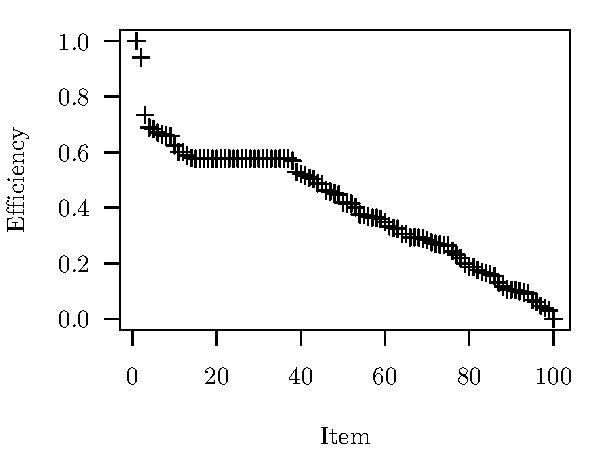
\includegraphics[width=0.42\textwidth]{figs/dcases=0.pdf}
	\label{fig:originaleff}
	}
	\subfigure[Efficiencies rounded to one decimal case.]{
	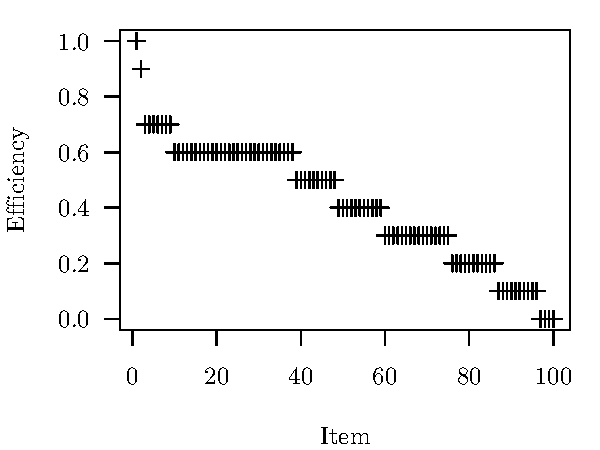
\includegraphics[width=0.42\textwidth]{figs/dcases=1.pdf}
	\label{fig:roundedeff}
	}
	\caption{Efficiency groups produced by rounding the original efficiencies to one decimal case.}
\end{figure}


Figure~\ref{fig:roundedeff} shows us the same efficiencies but now rounded to the first decimal case ($d=1$). Rounding, as a pre-processing phase of the efficiencies, makes evident other plateaus, each of them indicating a group of items whose efficiencies are approximately the same, i.e. an \textit{efficiency group}. Therefore, the number of decimal cases kept during the rounding allows us to roughly control the sizes of the groups. In summary, an \textit{efficiency group} is a subset of items of cardinality higher than one whose efficiencies are equal. Given that an efficiency group contains only items of similar efficiencies, the randomization of their order will not lead to massive deterioration of the heuristic information provided by the efficiencies. Therefore, efficiency groups enable an effective exploration of the space of orderings during the search for solutions. 


\section{Methodology}\label{sec:methodology}

In this paper, we evaluate the possible benefits of two simple randomizing operators that modify the positioning of items in a efficiency group given an ordering $\Ord^\text{dual}$.

\begin{description}
\item[Random-group swap ({\sc rg-swap}).] Randomly chooses an efficiency group, swap the positions of two randomly chosen items in the group.
\item[Random-group shuffle ({\sc rg-shuffle}).] Randomly chooses an efficiency group, shuffles the positions of all its items.
\end{description}

To verify the effectiveness of these operators we must first decide how frequently randomization should take place. Since the \gls{CBGA} is an effective algorithm to find high-quality solutions fast, the use of intensive randomization during the first generations would slow-down its progress. To avoid this drawback, we can associate the exploration of new orderings with the number of improving solutions produced by the heuristic repair during a generation. In other words, whenever an ordering ceases to produce improving solutions, randomization will be activated. Next section, describes a modified version of the \gls{CBGA} that implements such strategy.

%
%
%
%	The Chu & Beasley Genetic Algorithm
%
%
%
\subsection{Chu \& Beasley GA with efficiency groups}\label{sec:cbga}
\newcommand{\p}{\mathcal{P}}
The \gls{CBGA} uses a direct representation (binary strings), binary tournament selection, standard uniform crossover, random mutation of two bits and the heuristic repair (see Algorithm~\ref{alg:cbga-generation}).  

\begin{algorithm}[h!t]
	\caption{{\tt CBGA-newsolution($\p$)}}
	\label{alg:cbga-newsolution}
	\begin{algorithmic}[1]
	   \State Select $\x^1\in\p$ by a binary tournament 
	  \State Select $\x^2\in\p$ by a binary tournament 
	   \State $\x\leftarrow$ \texttt{uniformCrossover($\x^1$, $\x^2$)}
	   \State \texttt{flipTwoBits($\x^3$)}
		\State \Return $\x$.		
	\end{algorithmic}
\end{algorithm}

\gls{CBGA} is a steady-state algorithm, which means it generates and evaluates one solution at the time. However, to control the activation of the randomization of efficiency orderings, we must have access to the number of improving solutions produced. Therefore, we redesigned the \gls{CBGA} regarding generations, every generation consisting of $N$ attempts to produce improving solutions (where $N$ is the population size). Each of such attempts produces one solution $\x$ and applies the heuristic repair to it. The resulting solution is an improvement if it is both unique and better than the worst solution in $\p$ (see Algorithm~\ref{alg:cbga-generation}).

\begin{algorithm}[h!t]
	\caption{{\tt CBGA-generation}($\p, N, \Ord^\text{dual}$)}
	\label{alg:cbga-generation}
	\begin{algorithmic}[1]	
		\State $m \gets 0$
		\State improvements $\gets 0$
		\While{$m < N$}
			   \State $\x\gets$ {\tt CBGA-newsolution($\p$)}
			   \State {\tt heuristic-repair}($\x$, $\Ord^\text{dual}$)
			   \If {$\x$ is unique and better than the worst solution in $\p$} 
			   	\State $\x$ substitutes the worst solution in $\p$
			   	\State improvements $\gets$ improvements $+ 1$
			   \EndIf
			   \State $m \gets m + 1$
		\EndWhile
		\State \Return improvements.		
	\end{algorithmic}
\end{algorithm}

The modified version of the \gls{CBGA} that supports the randomization of efficiency groups is defined by Algorithm~\ref{alg:cbga}, which we will refer to as \CBGAe, where $d$ refers to the number of decimal cases used to round the efficiencies. The first step is to sort the indexes of the items in non-increasing order according to $e^\text{dual}$. Next, the efficiency groups are identified and stored in $g$. A population $\p$ of $N$ random candidate solutions is generated. All candidate solutions undergo heuristic repair and the search starts. At every generation, if no improving solutions are produced, the randomization of the ordering takes place (where {\tt rand-ordering} is a placeholder for {\sc rg-swap} or {\sc rg-shuffle}). 

\begin{algorithm}[h!t]
	\caption{\CBGAe}
	\label{alg:cbga}
	\begin{algorithmic}[1]
		\Require The population size $N$
		\State $\Ord^\text{dual}\leftarrow$ \texttt{sort($\{1,\dots,n\}$, $e^\text{dual}$)} 
		\State $g \gets $ {\tt get-efficiency-groups}($\Ord^\text{dual}, d$)
		\State Generates $N$ random candidate solutions in $\p$

		\State {\tt heuristic-repair}($\x$, $\Ord^\text{dual}$), $\forall \x\in\p$
		
		
		\While{Stop criteria not met}			
			   \State $m \gets $ {\tt CBGA-generation}($\p$, $N$, $\Ord^\text{dual}$)
			   \IfThen {$m \leq 0$} {{\tt rand-ordering}($\Ord^\text{dual}$, $g$)}
		\EndWhile
		\State \Return the best solution in $\p$.		
	\end{algorithmic}
\end{algorithm}



%
%
%
%								EXPERIMENTS
%
%
%
\subsection{Experiments}

The instances provided by \cite{chu1998} have been widely used in the literature and will be also the basis for our experiments. The set comprises instances of size $n\in\{100,250,500\}$, for each size there are instances of dimension $m\in\{5,10,30\}$ and tightness ratio $\alpha\in\{0.25,0.5,0.75\}$ (where $\alpha=c_i/\sum_{j=1}^n w_{ij}$). For each tuple $(n, m, \alpha)$ there are $10$ instances, totalizing $270$ different instances. All these instances are available in the \Orlib web page\footnote{\url{http://people.brunel.ac.uk/~mastjjb/jeb/orlib/mknapinfo.html}}.




\input{xtables/5-100.xtable}
\input{xtables/5-250.xtable}
\input{xtables/5-500.xtable}

\input{xtables/10-100.xtable}
\input{xtables/10-250.xtable}
\input{xtables/10-500.xtable}
























%
%
%
%							Results
%
%
%
\section{Results and Discussion}\label{sec:results}
This section describes and compare the results of both scenarios previously defined. We first show the  average performance of each algorithm in all $270$ Chu and Beasley instances. The averages were computed considering the whole set of instances, instead of separating instances according to their $\alpha$. This decision enables us to see the big picture of average performances of the algorithms and, since the same instances were used for all algorithms, the averages provide a relevant estimate for the performance measures used.
%
%
%
%				GAP
%
%



%
%
%							Conclusions
%
%
%
%\glsresetall
\section{Conclusion}\label{sec:conclusions}


%
%
%
%			Bibliography
%
%
\bibliographystyle{model5-names}
\bibliography{tudo}

\end{document}



